\chapter{Temperature sensor conditioning circuit}\label{sec:temp_sensor}

%**********************************************
\section{Intro} \label{sec:temp_intro}
%**********************************************
The signal obtained from the temperature sensor presents as DC, with a \SI{35}{\milli \volt}, \SI{50}{Hz} AC signal superimposed, which serves no purpose, but creates noise. The DC component increases linearly with respect to the temperature measured by the sensor. However, the sensor outputs a voltage of \SI{440}{\milli \volt} at 0\degree C, which increases by \SI{35}{\milli \volt} for every 1\degree C. These voltage levels are too small for a microcontroller ADC to take as input. Furthermore, as the sensor is only meant to measure human body temperature, the applicable range is only from 34\degree C to 42\degree C. The two aforementioned considerations necessitate amplification of the relevant part of the temperature sensor signal to occupy as much of a \numrange{0}{5} \si{\volt} range as possible, as this is the voltage range used by the ADC.
To this end, a temperature sensor conditioning circuit is required to transform the given input into the desired output. This conditioning circuit consists of a filter, an offset removing subcircuit, as well as an amplifier. The filter attenuates the AC signal present in the input signal in order to obtain an output signal with a minimal amount of noise. The offset removing subcircuit removes enough of the DC offset to ensure that the output signal is centered around \SI{2.5}{\volt}, which is necessary to obtain the largest possible output swing as discussed previously. Finally, the amplifier increases the magnitude of the input signal in order to be suitable as input for an ADC.

%**********************************************
\section{Design}\label{sec:temp_design}
%**********************************************
The amplifier was designed first, as its gain serves as the determining factor for the amount of noise reduction that is required from the filter. A TLC2272 op-amp was chosen as it allows for an output very close to its rails. Since the output signal has to be centered around \SI{2.5}{\volt}, a differential amplifier was decided upon, as the negative input can be used to adjust the offset present in the output. Given a zero-reference temperature sensor voltage ($V_{zero}$) of \SI{440}{\milli \volt}, with an increase ($V_{\Delta}$) of \SI{35}{\milli \volt} for every 1\degree C. Therefore, temperature sensor voltage levels are calculated as follows: $V_{temp} = V_{zero} + V_{\Delta} \times \mathrm{Temp}$ 

%Table \ref{tab:temp} shows some of the relevant voltage levels:

\begin{table}[h]
        \centering
        \footnotesize
        \caption{Temperatures and Corresponding Voltage Levels}
         \begin{tabular}{c@{\qquad}rrr}
          \toprule
          Temperature [\degree C] 	& 32    & 38	& 42\\
          Voltage [V] 			& 1.63	& 1.77	& 1.91\\
          \bottomrule
        \end{tabular}
     \label{tab:temp}
\end{table}

According to table \ref{tab:temp}, the maximum input voltage swing equals $1.91 - 1.63 = 0.28$V, and has a DC offset of \SI{1.77}{\volt}. Amplification is needed to reach an output voltage swing of \SI{5}{\volt}. Therefore:

$$A_v = \frac{V_{out}}{V_{in}} = \frac{5}{0.28} = 17.86$$

Now, R is selected as \SI{10}{\kilo \Omega}, to prevent a large current from being drawn.  This gives $R_{feedback} = 178.6$k$\Omega$, according to $A_v = \frac{{R}_{feedback}}{R}$ \cite{opamp}. R corresponds to $R_1$ and $R_2$, and $R_{feedback}$ to $R_{3}$ and $R_4$ in the final design diagram (figure \ref{fig:final}), which is shown here already to aid with the explanation of the design process. 

\begin{figure}[H]
    \centering
    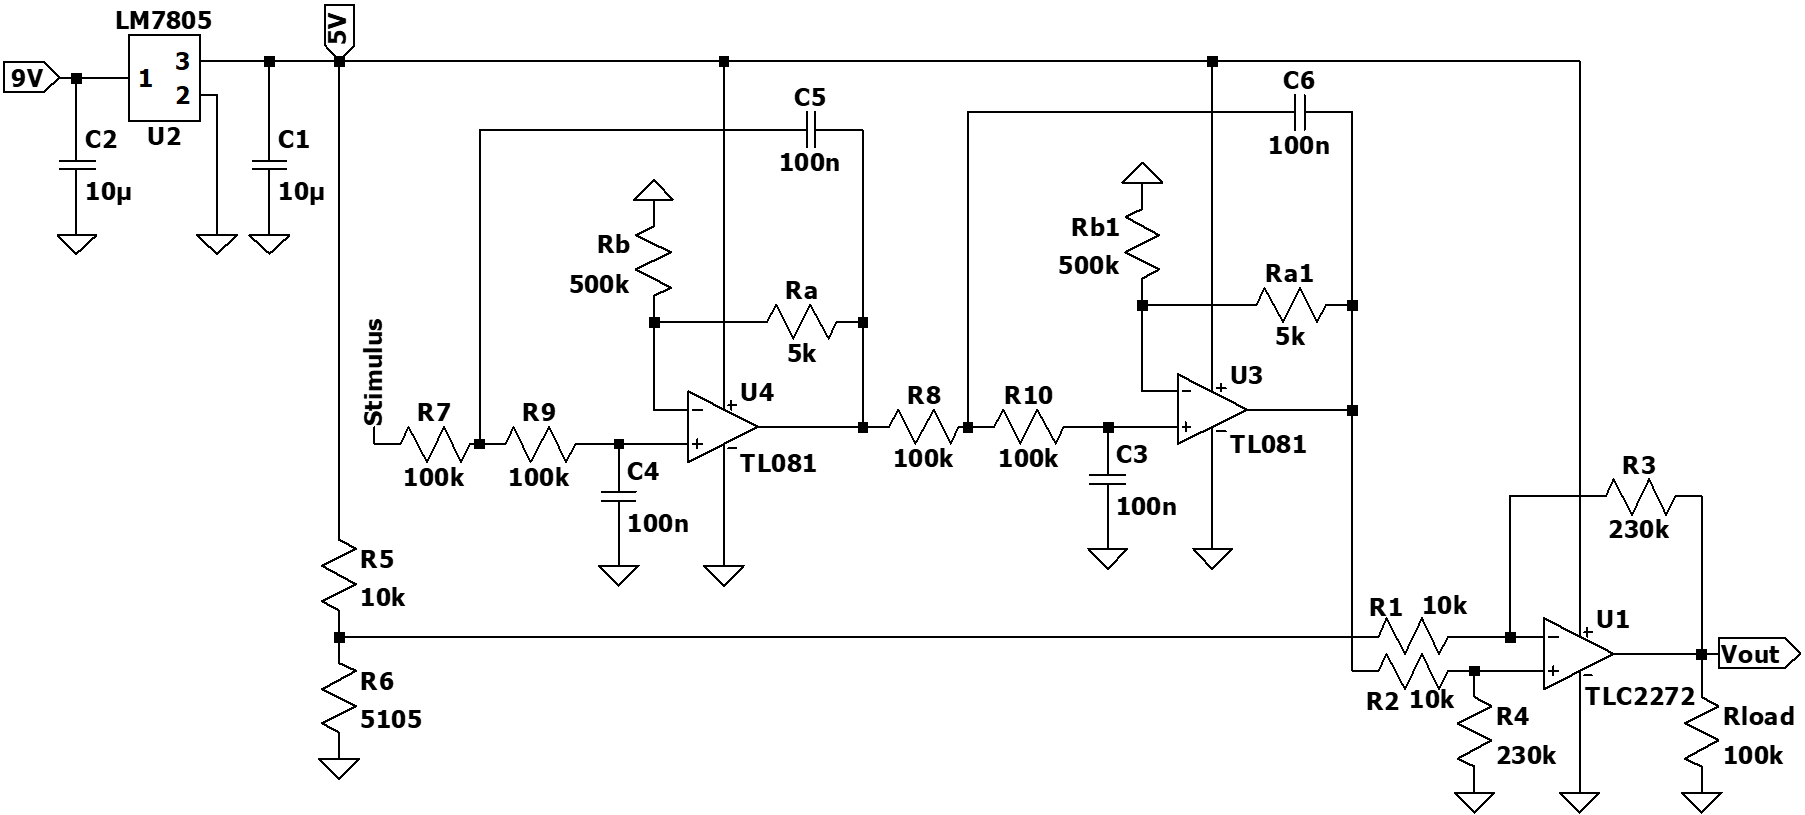
\includegraphics[width = 1\textwidth]{Figures/final.png}
    \caption{Temperature Sensor Circuit}
    \label{fig:final}
\end{figure}

Two points need to be considered: 
\begin{enumerate}
\item The DC offset of the input signal is undesired and has to be removed in order to obtain a zero-mean input signal. This can be achieved by designing another subcircuit that makes use of another op-amp, for example. This adds to the cost and complexity of the circuit.
\item The output signal has to be centered around \SI{2.5}{\volt}. This means that a DC offset has to be added in the form of a virtual ground.
\end{enumerate}

When considered in conjunction with each other, the DC offset alteration can be resolved in one step, thereby reducing cost and complexity significantly. The decision was therefore made to use a differential amplifier, with the input signal connected to the positive input, after which the voltage required at the negative input can be calculated in such a way as to simultaneously subtract the offset and add the virtual ground in one step, thereby producing an output DC offset of \SI{2.5}{\volt} (the lecturer mentions that this is an acceptable approach in Lecture Video 2).  This approach also simplifies the design procedure, as it becomes unnecessary to calculate the virtual ground separately. The differential amplifier, however, has to be non-inverting. The calculation thus reduces to a simple differential amplifier gain formula \cite{opamp}: 

$$V_{out}=\frac{{R}_{feedback}}{{R}}\left({V}_{in+}-{V}_{in-}\right) \;\;\; \rightarrow \;\;\; 2.5=\frac{178600}{10000}\left(1.77-{V}_{in-}\right)$$

With $V_{out}$ as \SI{2.5}{\volt}, $V_{in+}$ as \SI{1.77}{\volt} and the resistor values as calculated previously, ${V}_{in-} = 1.63 \; \mathrm{V}$. The voltage at ${V}_{in-}$ can be set by means of a voltage divider circuit, which takes \SI{5}{\volt} as input and is calculated as follows (resistor names in formulae are selected to conform with Figure \ref{fig:final}):

$${V}_{in-} = 5 (\frac{R_{6}}{R_{6}\times R_{5}})$$

Selecting $R_5$ as \SI{10}{\kilo \Omega} gives $R_6 =$ \SI{4.84}{\kilo \Omega}.\\

The filter has to be designed next. Possible design choices included an active/passive first order low-pass filter, a simple RC filter, or a second order low-pass filter. Simulation of the aforementioned filters has shown the following: the RC filter is very simple, but does not meet the design requirements w.r.t. noise. The passive low-pass filter is relatively simple, but does not meet the settling time requirement. The active low-pass filter meets both the noise and settling time requirements, but requires the TLC2272 op-amp to do so. Since a single TLC2272 op-amp is more expensive than multiple TL081 op-amps, the decision was made to rather use cascaded second order low-pass filters, which  make use of the TL081. This is somewhat more complex, but lowers the cost, as the final circuit now only uses three op-amps, two of which are the cheaper TL081 models. The cascaded setup also produces an output signal with extremely low noise.  A filter gain of close to unity is desired; for $R_A = $ \SI{500}{\kilo\Omega}, a value of \SI{5}{\kilo\Omega} is suitable for $R_A$, according to the formula from \cite{filter}:

$${A_v}=1+\frac{{R}_A}{R_B}$$

The settling time requirement of \SI{100}{ms} means that a cutoff frequency of more than \SI{10}{Hz} is needed, while the attenuation of noise requires a cutoff frequency below \SI{50}{Hz}. In order to minimize noise, the cutoff frequency was selected at \SI{15}{Hz}. Choosing R ($\mathrm{R_7 \; and \; R_9}$ in the diagram) as \SI{100}{\kilo\Omega} gives C ($\mathrm{C_4 \; and \; C_5}$) as \SI{106.1}{nF}, according to

$$f_c=\frac{1}{2 \pi RC}$$

This filter is then duplicated and connected back-to-back in order to form cascaded second-order low-pass filters, as seen in figure \ref{fig:final}.\\

Under most circumstances, it is a good design practice to include a unity gain op-amp at the input of the op-amp responsible for the correct offset, as it acts as a voltage buffer, thereby clamping the voltage against fluctuations caused by the differential amplifier's other input. This design practice was considered, but ultimately decided against, as tests with and without the buffer provided outputs of equal quality (similar to the output shown in section \ref{sec:temp_results}. The only notable differences resulting from the inclusion of a buffer were an increase in current drawn, as well as an increase in cost for the circuit components, as another op-amp is required. Therefore, in order to keep the current consumption below \SI{15}{mA}, as well as to use reduce cost by only using three op-amps, the voltage buffer was omitted in the final design. 


%**********************************************
\section{Results} \label{sec:temp_results}
%**********************************************
The designed circuit produces a signal centered at \SI{2.5}{\volt} with an output swing of \SI{4.86}{\volt}, exceeding the required \SI{3.5}{\volt}. The absolute maximum amount of noise measured is \SI{25.6}{\milli\volt}, and the settling time is \SI{67}{ms}, thereby meeting the requirements of \SI{50}{\milli\volt} and \SI{100}{ms} respectively. Total current draw is \SI{12.83}{mA}, well below the required \SI{15}{mA}. Measurements and graphs of settling time, cutoff frequency and current drawn can be seen in Appendix C. It is thus clear that all requirements, as well as all bonus requirements, have been met with a good margin to spare, all the while using only three op-amps, two of which are the cheaper TL081 models. The output signal (light blue) is shown in figure \ref{fig:vout}.

\begin{figure}[h]
    \centering
    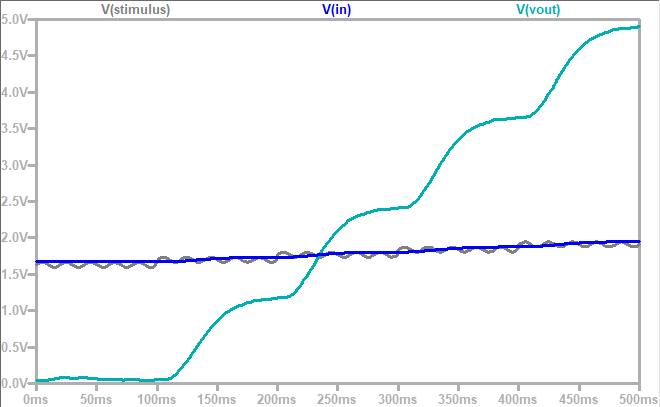
\includegraphics[width = 1\textwidth]{Figures/vout.png}
    \caption{Temperature Sensor Conditioning Circuit Output}
    \label{fig:vout}
\end{figure}

%**********************************************
\section{Summary}\label{sec:temp_summary}
%**********************************************
Concluding, the circuit performs very well, and successfully amplifies the temperature sensor output to a level that is readable by the microcontroller ADC, all the while attenuating almost all noise present in the input. The design is somewhat complex, but also cheaper, as it uses less of the TLC2272 op-amps.


